\documentclass[a4paper,12pt]{article}

%%% Работа с русским языком
\usepackage{cmap}					% поиск в PDF
\usepackage{mathtext} 				% русские буквы в формулах
\usepackage[T2A]{fontenc}			% кодировка
\usepackage[utf8]{inputenc}			% кодировка исходного текста
\usepackage[english,russian]{babel}	% локализация и переносы

%%% Дополнительная работа с математикой
\usepackage{amsmath,amsfonts,amssymb,amsthm,mathtools} % AMS
\usepackage{icomma} % "Умная" запятая: $0,2$ --- число, $0, 2$ --- перечисление

%% Номера формул
%\mathtoolsset{showonlyrefs=true} % Показывать номера только у тех формул, на которые есть \eqref{} в тексте.
%\usepackage{leqno} % Нумерация формул слева

%% Свои команды
\DeclareMathOperator{\sgn}{\mathop{sgn}}

%% Перенос знаков в формулах (по Львовскому)
\newcommand*{\hm}[1]{#1\nobreak\discretionary{}
{\hbox{$\mathsurround=0pt #1$}}{}}

%%% Работа с картинками
\usepackage{graphicx}  % Для вставки рисунков
%%\graphicspath{{images/}{images2/}}  % папки с картинками
\setlength\fboxsep{3pt} % Отступ рамки \fbox{} от рисунка
\setlength\fboxrule{1pt} % Толщина линий рамки \fbox{}
\usepackage{wrapfig} % Обтекание рисунков текстом

%%% Работа с таблицами
\usepackage{array,tabularx,tabulary,booktabs} % Дополнительная работа с таблицами
\usepackage{longtable}  % Длинные таблицы
\usepackage{multirow} % Слияние строк в таблице

%%% Теоремы
\theoremstyle{plain} % Это стиль по умолчанию, его можно не переопределять.
\newtheorem{theorem}{Теорема}[section]
\newtheorem{proposition}[theorem]{Утверждение}
 
\theoremstyle{definition} % "Определение"
\newtheorem{corollary}{Следствие}[theorem]
\newtheorem{problem}{Задача}[section]
 
\theoremstyle{remark} % "Примечание"
\newtheorem*{nonum}{Решение}

%%% Программирование
\usepackage{etoolbox} % логические операторы

%%% Страница
\usepackage{extsizes} % Возможность сделать 14-й шрифт
\usepackage{geometry} % Простой способ задавать поля
	\geometry{top=25mm}
	\geometry{bottom=35mm}
	\geometry{left=35mm}
	\geometry{right=20mm}

%\usepackage{fancyhdr} % Колонтитулы
% 	\pagestyle{fancy}
 	%\renewcommand{\headrulewidth}{0pt}  % Толщина линейки, отчеркивающей верхний колонтитул
% 	\lfoot{Нижний левый}
% 	\rfoot{Нижний правый}
% 	\rhead{Верхний правый}
% 	\chead{Верхний в центре}
% 	\lhead{Верхний левый}
%	\cfoot{Нижний в центре} % По умолчанию здесь номер страницы

\usepackage{setspace} % Интерлиньяж
%\onehalfspacing % Интерлиньяж 1.5
%\doublespacing % Интерлиньяж 2
%\singlespacing % Интерлиньяж 1

\usepackage{lastpage} % Узнать, сколько всего страниц в документе.

\usepackage{soul} % Модификаторы начертания

\usepackage{hyperref}
\usepackage[usenames,dvipsnames,svgnames,table,rgb]{xcolor}
\hypersetup{				% Гиперссылки
    unicode=true,           % русские буквы в раздела PDF
    pdftitle={Заголовок},   % Заголовок
    pdfauthor={Автор},      % Автор
    pdfsubject={Тема},      % Тема
    pdfcreator={Создатель}, % Создатель
    pdfproducer={Производитель}, % Производитель
    pdfkeywords={keyword1} {key2} {key3}, % Ключевые слова
    colorlinks=true,       	% false: ссылки в рамках; true: цветные ссылки
    linkcolor=blue,          % внутренние ссылки
    citecolor=black,        % на библиографию
    filecolor=magenta,      % на файлы
    urlcolor=cyan           % на URL
}

\usepackage{cite} % Работа с библиографией
%\usepackage[superscript]{cite} % Ссылки в верхних индексах
%\usepackage[nocompress]{cite} % 
\usepackage{csquotes} % Еще инструменты для ссылок

\usepackage{multicol} % Несколько колонок

\author{Мария Ершова, БКЛ-173}
\title{Проект по Цифровой Граммостности}
\date{\today}

\begin{document} % конец преамбулы, начало документа

\maketitle

\tableofcontents

\section{Éire}

Is oileán í Éire atá suite amuigh ó chósta iarthuaisceart mhórthír na hEorpa, siar ón mBreatain Mhór, in oirthear an Aigéin Atlantaigh thuaidh.

\begin{figure}[h!]
\centering
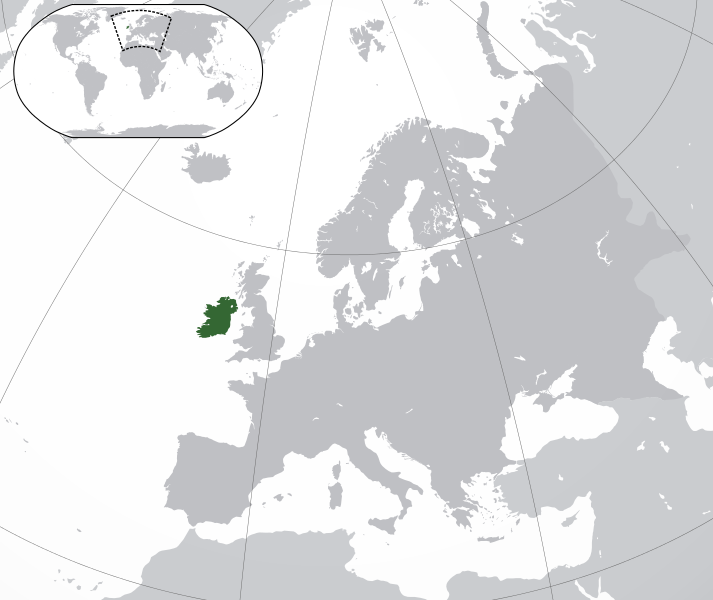
\includegraphics[width=0.6\linewidth]{Map_of_Ireland_in_Europe.png}
\caption{Suíomh an oileáin}
\end{figure}


\subsection{Rialtas}

Ó 1922 i leith, tá an t-oileán roinnte idir Saorstát Éireann (1922-1937) nó Éire (1937-inniu) agus Tuaisceart Éireann. Tá na sé chontae i dTuaisceart Éireann mar chuid den Ríocht Aontaithe, agus tá an chuid eile den tír ina Stát neamhspleách. Go minic freisin tugtar <<na sé chontae>> ar Thuaisceart Éireann, agus <<na sé chontae is fiche>> nó <<an Phoblacht>> ar an gcuid eile den tír.

\subsection{Daoine}

\begin{wrapfigure}{r}{0.4\linewidth}
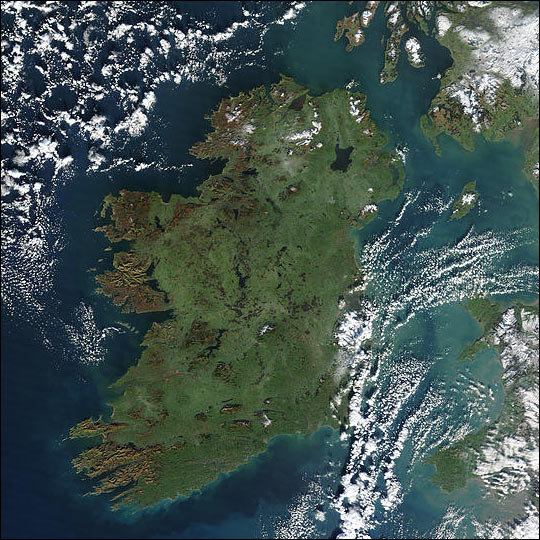
\includegraphics[width=\linewidth]{Ireland_NASA.jpg}
\caption{Íomhá Éireann i ndathanna cearta, déanta ag satailít NASA ar 4 Eanáir, 2003. Is féidir Alba, Oileán Mhanann agus an Bhreatain Bheag a fheiscint soir uaithi.}
\end{wrapfigure}Tá beagnach seacht milliún duine in Éirinn. Is de bhunadh Ceilteach an chuid is mó den daonra, a tháinig i dtír ó mhór-roinn na hEorpa thar na cianta. Bhí cuid mhaith inimirce, freisin, ó am go ham ó thíortha eile, go háirithe as Alba, agus ar bhonn níos lú, as Sasana. Is Caitlicigh formhór (os cionn 70\%) an daonra. Is Protastúnaigh formhór na coda eile, beagnach leath na ndaoine i gCúige Uladh, agus iad roinnte idir eaglaisí éagsúla, go háirithe Preispitéirigh agus Anglacaigh (a bhaineann le hEaglais na hÉireann. Féach ar an alt Creideamh in Éirinn le tuilleadh sonraí).

\subsection{Cultúr}

Tá cáil ar na Gaeil ó thús a gcuid staire sa cheol. Bhíodh ceoltóirí agus cumadóirí ceardúla go fairsing sa tír faoi na sean-ríthe agus flatha, go dtí gur chuir Cath Chionn tSáile deireadh leis an seanchóras Gaelach. As sin amach, leanadh den cheol, ach ba cheol tíre an chuid ba mhó de, le ceol rince agus oibre san áireamh.

Níos déanaí, tháinig foirm amhránaíochta gan tionlacan ar aghaidh, ar a dtugtar an seannós. Tá sé seo láidir fós, go háirithe i nGaeltachtaí Chonnacht. Tá traidisiúin ceol fidile láidir i gcuid mhór den tír, ach castar ceol traidisiúnta freisin ar an gcruit, ar an bhfeadóg stáin, agus ar an mbosca ceoil go forleathan. Bhíodh rincí traidisiúnta go rialta ag na crosbhóthair go dtí na 1950í, ach ina dhiaidh sin ba sna hallaí rince ba mhó a bhí ceol le haireachtáil go beo. Ar ndóigh chuir an disco tarraing i gcónra na mbannaí agus na hallaí ceoil, cé go leanann cuid acu go fóill.

Maraon leis an gceol, tá cáil ar na Gaeil leis an scríbhneoireacht. San fhichiú céad agus sa 21ú céad is i mBéarla atá an chuid is mó den scríbhneoireacht seo, ar aon dul leis an titim ar úsáid na Gaeilge thar an achar sin.

\subsection{Flóra agus fána}

Ós rud é go raibh an t-oileán scartha amach ó mhór-roinn na hEorpa de bharr ardú mara ag deireadh na hoighearaoise, níl a leithéid d'éagsúlacht ainmhithe is a bhfuil le fáil sa Bhreatain nó ar mhórthír na Eorpa. Na speicis a fhaightear go fliúrseach ná an sionnach, an ghráinneog agus an broc; chomh maith leis an giorria, an fia rua agus an cat crainn i líonanna níos lú. Tagtar ar roinnt ainmhíthe mara i bhfarraigí an oileáin freisin, mar atá an turtar mara, an siorc, an rón, an míol mór agus an deilf.
Níl nathair ar bith le fáil, agus is í an laghairt an t-aon reiptíl a fhaightear ann.
I measc na speicis díofa a chuaigh i léig ná an fia mór, an fhalcóg mhór agus an mac tíre. Tugadh an t-iolar fíréan isteach arís, tar éis dó a bheith imithe leis na glúinte.

\subsection{Spórt}

\begin{wrapfigure}{r}{0.4\linewidth}
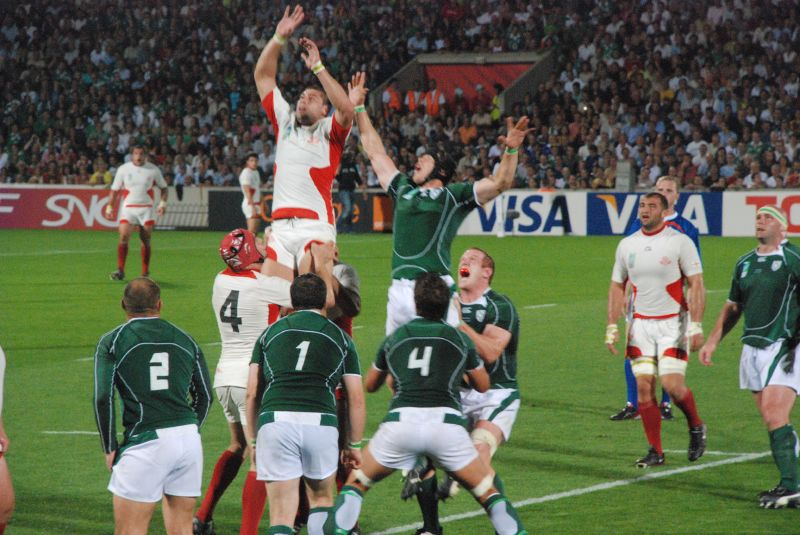
\includegraphics[width=\linewidth]{Ireland_vs_Georgia.jpg}
\caption{Foireann rugbaí náisiúnta na hÉireann ag imirt i gcoinne na Seoirsia (2007)}
\end{wrapfigure}Tá a gcluichí traidisiúnta féin ag na hÉireannaigh. Is iad iomáint, peil Ghaelach, camógaí agus liathróid láimhe na cluichí Gaelacha. Is é Cumann Lúthchleas Gael an eagraíocht atá i gceannas ar na cluichí seo. Tá suim ag go leor daoine sa sacar freisin, agus faigheann foireann sacair náisiúnta Phoblacht na hÉireann a lán tacaíochta inniu. Chomh maith leis sin, tá galf, snúcar agus rugbaí coitianta freisin. Imríonn foireann rugbaí náisiúnta na hÉireann (agus an Cumann Rugbaí na hÉireann) ar son an oiléain ar fad.

\subsection{Na meáin chumarsáide}

Tá an chuid is mó de na meáin i bPoblacht na hÉireann bunaithe i mBaile Átha Cliath. Is iad na príomhnuachtáin ansin an Irish Times, an Irish Independent, agus le cupla bliain anuas an Irish Examiner. Bhí an Cork Examiner ar an nuachtán seo ar feadh blianta, ach bheartaigh siad díol náisiúnta a thabhairt dó, agus athainmníodh mar sin é. Tá eagráin d'Éireann ag go leor de nuachtáin Shasana, ach is ionann formhór an ábhair. Tá díol leathan ar an Belfast Telegraph agus an Irish News as Béal Feirste, ach níl mórán díol nó glaoch orthu ó dheas go dtí seo. Bhí an Irish Press, Sunday Press agus Evening Herald an-tábhachtach go dtí na 1970í, agus iad á riaradh ag muintir Éamon de Valera. Tá nuachtáin ar leith a fhoilsítear ar an Domhnach, ar nós an Sunday Independent ó fhoilsitheoirí an Irish Independent, an Sunday World. Tá dhá nuachtán Gaeilge ann: Lá (atá laethúil, as Béal Feirste) agus Foinse (atá seachtainiúil, as An Cheathrú Rua).

Is é Radio Telefís Éireann an príomhchraoltóir ó dheas, le trí bealach teilifíse sa chuid is mó den tír: RTÉ a hAon, RTÉ a Dó agus TG4. Tá TV3 agus Channel 6 neamhspleách ón stát. Tá an BBC ag craoladh ón oirthuaisceart, chomh maith le hUTV atá neamhspleách ón rialtas ó thuaidh. Tá tábhacht fós leis na craoltóirí náisiúnta ar an dá thaobh den teorann, ach tá an-éisteacht anois le stáisiúin neamhspleácha.

\subsection{Stair}

Deirtear gurbh iad clanna Míle an slua mór deireanach a tháinig i dtír, is a thug an chuid is mó den chultúr Gaelach dúinn a bhfuil aithne fós air. Roimhe sin bhí grúpaí eile ann dar leis na seanscéalta, ar nós na bParthalónach, agus na bhFear Bolg.

Tháinig an Chríostaíocht go hÉirinn nuair a chuir an Pápa Ceilistín Palladius go hÉirinn in AD 430. Ach ba é Naomh Pádraig, saoránach Rómhánach de bhunadh Breatnach, ar éirigh leis an chreideamh nua a thabhairt go hÉirinn ó 432 ar aghaidh. Seachas mar a tharla i ngo leor tíortha eile, ní raibh aon chath mór i gceist, ach gur chloígh an eaglais sean-chreideamh na nGael diaidh ar ndiaidh.

Ní raibh tionchar mór díreach ag na Rómhánaigh ar Éirinn mar a bhí acu ar an gcuid eile d'iarthar na hEorpa. Ach bhí na Lochlannaigh is na Danair ag ionsaí na tíre ón 9ú aois, agus ba iad na Lochlannaigh a chuir tús le bailte móra na hÉireann, agus a rinne ruaigeanna ar na mainistreacha agus ar na tithe móra. Mar shampla, chuireadar Baile Átha Cliath ar bun i 841. Chuir na Gaeil le chéile ina dhiaidh sin, agus thoghadar an chéad Ard-Rí i 1003. Cé nach raibh cumhacht mhór aige, thógadh an rí ba láidre an teideal de ghnáth. Ag Cath Chluain Tarbh, chloígh na Gaeil slua Lochlann ar deireadh, cé gur maraíodh Brian Bóirmhe, ceannaire na nGael.

Sa 12ú haois, ba iad na Normanaigh a tháinig i dtír. Bhí Diarmuid Mac Murchadha Caomhánach san oirdheisceart i dtrioblóid lena chuid talún agus le tiarnaí eile sa chuid sin tíre, agus d'iarr sé cúnamh ar Rí Anraí II Shasana i 1171. Chuir Anraí Strongbow, tiarna Normanach ón mBreatain Beag, i gcúnamh air. Ach má tháinig, d'fhan na Normanaigh, agus cé gur iomaí cath a troideadh, de réir a chéile ghlac siad seilbh ar thailte agus caisleáin agus bailte na hÉireann. Do lean cumhacht na nGall in Éirinn, óir choinnigh fórsaí rí Shasana smacht ar an gcuid den tír timpeall ar Bhaile Átha Cliath, an baile is mó a bhí faoi smacht na Lochlannach agus na Normanach ina ndiaidh. Laistigh de dhá ghlún, bhí rialtas lárnach i mBaile Átha Cliath, faoi stiúir dhíreach rí Shasana. I 1297 cuireadh an chéad pharlaimint ar bun, ach b'iad siúd de shliocht Gallda amháin a thogh agus a shuigh sa pharlaimint sin. Ó thús an 14ú aois, bhí Gaelú le sonrú imeasc na nGall a bhí fanta in Éirinn, agus cuireadh Dlithe Chill Chainnigh i réim i 1366, a chuir scoilt idir Ghael agus Gall. I ré na dTeodar, cuireadh breis máistreacht ar an tír, agus i 1494 cuireadh Dlí Poynings i réim. Thug sé sin cead do Rí Shasana dlithe nua ó pharlaimint Bhaile Átha Cliath a chosc. I 1534 deineadh Tiarnaí Tánaiste de Iarlaí Chill Dara, agus i 1541 ghlac rí Shasana an teideal "Rí na hÉireann" chomh maith. Sna blianta a lean, cuireadh brú ar na tiarnaí Gaelacha a dtailte a bhronnadh ar rí Shasana, ionas go dtabharfaí ar ais dóibh é mar dheontas ríoga, agus teideal Gallda ag dul leis. Ar ndóigh, chuaigh sé seo i gcoinne ghnás na nGael go mór, ach de réir a chéile ghlac go leor leis an réiteach seo.

De réir a chéile, leath cumhacht Shasana ón bPáil ar fud na tíre, trí chathanna, géilleadh na dtiarnaí Gaelacha don Choróin, agus le cur fúthu ag tiarnaí agus móraibh eile Sasanacha.

Ba é Cath Chionn tSáile i 1601 an iarracht mhór deiridh a rinneadh leis na Gaill a ruaigeadh as Éirinn. Bhí an baile i seilbh na Spáinneach, ach bhí ar arm na nGael teacht aduaidh ó chúige Uladh i lár an gheimhridh agus bhí an bua ag na Sasanaigh orthu. Tar éis Chath Chionn tSáile, thréig formhór na dtiarnaí Gaelacha an tír mar go raibh deireadh bunúsach leis an gcóras Gaelach, iTeitheadh na nIarlaí. D'imigh siad leo go dtí an mhór-roinn, go háirithe don Fhrainc agus don Spáinn. Ina dhiaidh sin ba de bhunadh Sasanach a bhí tiarnas na tíre, agus bhí na gnáthdhaoine an-bhocht.

Bhí tionchar mór ag Cogadh Cathartha Shasana, idir an rí agus lucht na parlaiminte, ar Éirinn i rith na 1640í. Buaileadh taobh an rí ar deireadh, agus cuireadh an Rí Séarlas I Shasana, chun báis ar 30 Eanáir, 1649. Tháinig Oilibhéar Cromail go Éirinn ar 15 Lúnasa 1649 mar rialóir míleata agus síbhialta na Parlaiminte le smacht a chur ar an tír. Cuimhnítear air go háirithe mar gheall ar an slad a dhein sé i nDroichead Átha ar an 11 Meán Fómhair 1649 agus i mbaile Loch Garman ar an 11 Deireadh Fómhair 1649. Tar éis do Chill Chainnigh géilleadh dó ar 27 Márta 1650, d'fhág sé an tír ar 25 Bealtaine, 1650.

Faoin mbliain 1660, tugadh parlaimint Bhaile Átha Chliath chun saoil arís, agus tháinig an Rí Séarlas II Shasana i gcoróin. Deineadh an chuid is mó den choilíniú in Éirinn i rith an 17ú céad. Cuireadh tiarnas Protastúnach, de bhunadh Sasanach, i seilbh ar an gcuid is mó agus is fearr de thailte na hÉireann, agus is acu freisin a bhí an chuid is fearr de na gnóthaí sna bailte freisin. Ón 17ú hAois go deireadh an 18ú haois, bhí na Péindlíthe nó na Dlíthe Peannadacha, a rinne leatrom ar Chaitlicigh agus Preisbitéirigh i bhfeidhm, cé nár imigh a rian go ceann i bhfad ina dhiaidh seo.

Tháinig an Rí Séamus II Shasana (Séamus a 'Chaca) i réimeas i 1685, ach i 1688 tháinig Liam Oráisteach i dtír i Sasana. I 1689 tháinig Séamus go hÉireann tar éis dó a bheith ar a theitheadh sa bhFrainc. I 1690 tháinig Liam go hÉireann, agus bhuail sé fórsaí Shéamuis ag Cath na Bóinne ar 1ú Iúil 1690, nó sa bhféilire nua, ar an 12ú Iúil, an lá a dhéanann an Ord Óráiste ceiliúradh ar an gcath. Bhuail fórsaí Liam cinna Shéamuis arís i 1691, ag Cath Eachdhroime, agus ag Conradh Luimní, conradh a bhfuil cáil air mar chonradh nár comhlíonadh, ghéill Pádraig Sáirséal, ar thaobh Shéamuis agus na nGael, d'fhórsaí Liam.

Deineadh iarracht ar leith ar an gcoilíniú i gcúige Uladh, tré mórán gnáth-Shasanaigh agus gnáth-Albanaigh a thabhairt isteach agus seilbh a thabhairt dóibh ar thailte sa chúige sin. Is as sin a leanann méid an phobail Aontachtach (go príomha Protastúnaigh) sa chúige sin, agus féachann siad siar fós go Cath na Bóinne, mar gurb é bua an Rí Liam ar Rí Séamus a thug tús áite don Phrotastúnachas i Sasana agus in Éirinn.

Ag deireadh an 18ú chéid, leath tuairimí an Soilsiú ón Mór-Roinn, tuairimí a bhí daonlathach agus poblachtach seachas bheith ag brath ar chumhacht an rí. Mar chuid de sin, bhí an-chaint ar na tuairimí seo imeasc cuid de lucht ceannais na tíre agus daoine eile le scolaíocht. D'aontóidís idir Chaitlicigh, Phrotastúnaigh agus Easaontóirí i náisiún amháin. Bhí sé seo tábhachtach san Éirí Amach i 1798, agus cé gur i gcoinne smacht Gallda a bhí sé, ba Phrotastúnaigh de bhunadh Sasanach cuid mhaith de na ceannairí. Bhí aighneas i gContae Loch Garman, m.sh. Cath Chnoc Fíodh na gCaor lámh le hInis Córthaidh. I gContae Mhaigh Eo d'éirigh chomh maith leis an aiséirí le cuidiú Francach gur tugadh Rásaí Chaisleáin an Bharraigh ar theitheadh na nGall. Ní hamháin nár éirigh leis an éirí amach, ach reachtáladh Acht an Aontais i 1800 i bparlaimint Bhaile Átha Cliath, rud a chuir deireadh leis féin.

Bhí na Péindlíthe fós i réim in Éirinn, agus cé nár cuireadh i bhfeidh iad mórán faoin am seo, chuir siad coscanna ar Chaitlicigh go háirithe. Bhí Domhnall Ó Conaill, a bhí ina theachta parlaiminte, an-ghníomhach sa troid le haghaidh comhrom na féinne a thabhairt do ghnáthmhuintir na tíre, a bhí an-bhocht agus arbh Chaitlicigh iad don chuid is mó. Reachtáladh an Acht Um Shaoirse Chaitliceach sa mbliain 1829 a thug ceart do Chaitlicigh bheith ina dteachtaí parlaiminte, agus glacadh le hoifigí sa saol cathartha agus míleata.
I rith an 19ú haois, bhí aighneas ar son na saoirse ó am go ham. Bhí éirí amach in 1803, agus múchadh go héasca é, agus cuireadh an ceannaire, Robert Emmet, chun báis. Timpeall na bliana 1845 a chuir Michael Davitt ón Sráid i gContae Mhaigh Eo Conradh na Talún ar bun. Is é a bhí á iarraidh acu ná cíos cothrom, ceart seilbh agus cead díolta. Bhí Conradh na Talún ar bun ar fud na tíre. Bhí Éirí Amach freisin in 1848. Theip ar an éirí amach sin, mar a theip ar gach ceann roimhe.

Ag deireadh an 19ú Aois, bhí Páirtí Parlaiminteach na hÉireann (Irish Parliamentary Party) gníomhach ag lorg saoirse don tír. Ba é Charles Stewart Parnell a bhí ina fheighil ar feadh i bhfad, ach nuair a cuireadh cairdeas a bhí aige le bean pósta Kitty O'Shea, ina leith, chuaigh an eaglais Chaitliceach ina choinne, agus uaidh sin thréig muintir na tíre é, gur chaill sé a cheannaireacht i 1890. Ina dhiaidh siúd, bhí John Redmond i bhfeighil ar an bpáirtí, agus lean siad go dtí gur éirigh le Sinn Féin uimhir mór feisirí a thoghadh i 1917, tar éis Éirí Amach na Cásca i 1916. Ní raibh ag páirtí Redmond ach seachtar fheisire, an chuid is-mó in Uladh (ceann amháin i Learpholl).
Chuir Sinn Féin an Chéad Dáil ar bun i 1918 i mBaile Átha Cliath mar gur acu a bhí bunús na bhfeisirí a toghadh go parlaimint Londain. Reachtáladh Acht Rialtais Éireann i Londain i 1920, agus cé go raibh saoirse d'Éireann i gceist, deir R.F. Foster ina leabhar, Modern Ireland, go raibh sé an-soiléir go mbeadh críochdheighilt freisin, mar go raibh rogha le bheith ag muintir an oirthuaiscirt gan a bheith páirteach sa neamhspleáchas. Go deimhin, cé go ndeachaigh an Bille um Riail Baile tríd an dteach íochtarach i Sasana i 1914, chuir Teach na dTiarnaí an oireadh athraithe air nár féadadh é a thabhairt i gcrích.

Ina dhiaidh seo, thosaigh Cogadh na Saoirse a lean go dtí an Conradh Angla-Éireannach i 1919. Ach ní raibh aontas faoin gconradh, mar gur aithin sé críochdheighilt na tíre, agus as seo a tháinig an Cogadh Cathartha nó Cogadh na gCarad, a bhí chomh crua céanna le Cogadh na Saoirse. Ach buaileadh an taobh Poblachtach a chuir i gcoinne an Chonartha, agus bhí rialtas neamhspleách anois sna 26 chontaethe ó dheas. Tá na sé chontaethe ó oir-thuaidh sa Ríocht Aontaithe ó shoin, i ríocht Thuaisceart Éireann.

\subsection{Tíreolaíocht}

\begin{wrapfigure}{r}{0.3\linewidth}
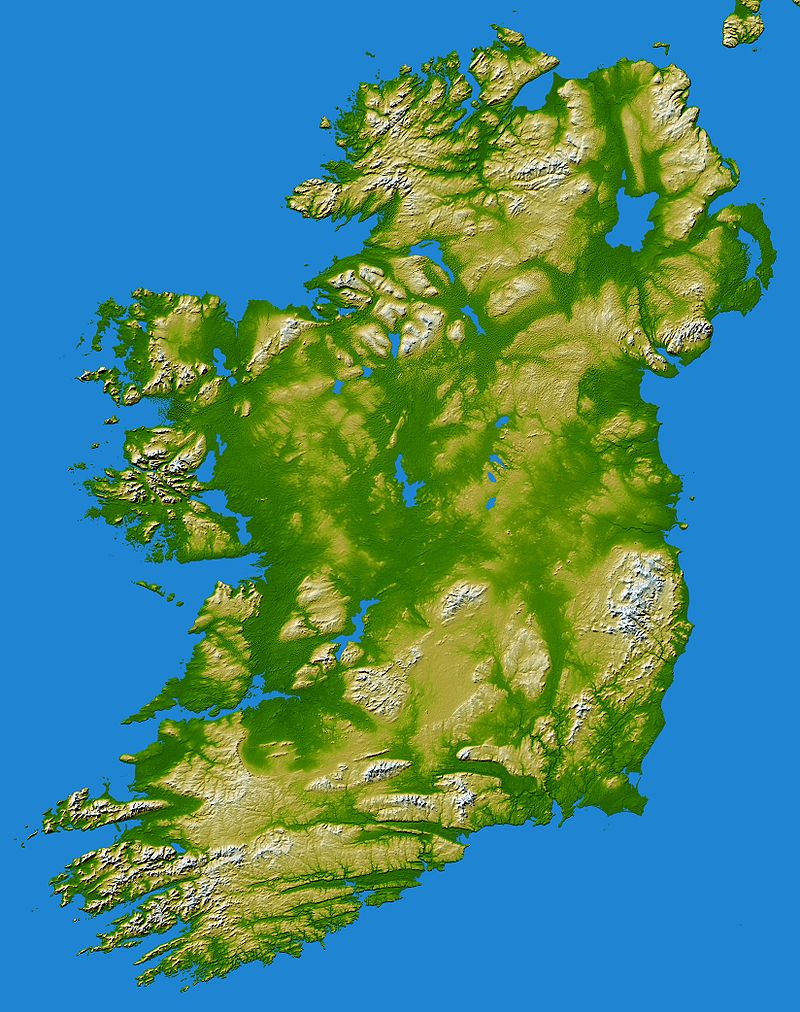
\includegraphics[width=\linewidth]{Topography_Ireland.jpg}
\caption{Topagrafaíocht}
\end{wrapfigure}Labhraítear go minic sa Ghaeilge ar Leath Mhogha agus Leath Choinn. Clúdaíonn leath Mhogha an cuid tíre atá ó dheas ó Eiscir Riada, agus Leath Choinn an chuid eile.

Tá an tír, ar ar thug na Rómhánaigh Hibernia, 486 ciliméadar (301 míle) ó thuaidh aneas, agus 275 ciliméadar (171 míle) anoir aniar. Tá maigheanna móra i lár na tíre, cuid mhaith díobh clúdaithe le portaigh, agus tá an-chuid cnoic agus sléibhte mórthimpeall orthu, ach níl mórán acu an-ard. Is é Corrán Tuathail i gContae Chiarraí an ceann is airde (1041 méadar).

Tá talamh mhaith san oirthear in áiteanna, agus déantar an-chuid curadóireachta, mar shampla ar chruithneacht, eorna, biatas siúcra agus torthaí. San iarthar, níl an oiread sin curadóireachta, mar go bhfuil an aeráid agus an talamh tais cuid mhór den bhliain, agus an talamh níos boichte i go leor áiteanna. Tógáil eallach agus caorach, maraon le ba bainne, an sórt talmhaíochta a chleachtaítear ansin don chuid is mó. Fanann siadsan amuigh faoin aer an bhliain ar fad de ghnáth, mar níl an aimsir in Éirinn chomh crua le tíortha eile i dTuaisceart na hEorpa mar gheall ar Shruth Murascaille Mheicsiceo. Féach Bóithre agus mótarbhealaí in Éirinn mar tuilleadh eolais faoi na bóithre agus na mótarbhealaí ar fháil in Éirinn.

\begin{itemize}
	\item Cúige Uladh (Tá sé chondae in Uladh fós faoi dhlínse na Breataine) 
	\begin{itemize}
		\item Contae Aontroma
		\item Contae Ard Mhacha
		\item Contae an Chabháin (san Phoblacht)
		\item Contae Dhoire
		\item Contae an Dúin
		\item Contae Dhún na nGall (P)
		\item Contae Fhear Manach
		\item Contae Mhuineacháin (P)
		\item Contae Thír Eoghain
	\end{itemize}
	\item Cúige Laighean
	\begin{itemize}
		\item Contae Átha Cliath 
		\begin{itemize}
			\item (Contae Átha Cliath Theas)
			\item (Cathair Bhaile Átha Cliath)
			\item (Contae Dhún Laoghaire - Ráth an Dúin)
			\item (Contae Fhine Ghall)
		\end{itemize}
		\item Contae Cheatharlach
		\item Contae Chill Chainnigh
		\item Contae Chill Dara
		\item Contae Chill Mhantáin
		\item Contae na hIarmhí
		\item Contae Laoise
		\item Contae Loch Garman
		\item Contae an Longfoirt
		\item Contae Lú
		\item Contae na Mí
		\item Contae Uíbh Fhailí
	\end{itemize}
	\item Cúige Chonnacht
	\begin{itemize}
		\item Contae na Gaillimhe
		\item Contae Liatroma
		\item Contae Mhaigh Eo
		\item Contae Ros Comáin
		\item Contae Shligigh
	\end{itemize}
	\item Cúige Mumhan 
	\begin{itemize}
		\item Contae an Chláir
		\item Contae Chorcaí
		\item Contae Chiarraí
		\item Contae Luimnigh
		\item Contae Phort Láirge
		\item Contae Thiobraid Árann 
		\begin{itemize}
			\item (Tiobraid Árann Thuaidh)
			\item (Tiobraid Árann Theas)
		\end{itemize}
	\end{itemize}
\end{itemize}

\subsubsection{Oileáin na hÉireann}
\begin{enumerate}
	\item Acaill
	\item Inis Bó Finne
	\item Inis Mór
	\item Inis Meáin
	\item Inis Oírr
	\item Toraigh
	\item Gabhla
	\item Reachrainn
	\item Reachlainn
	\item An Blascaod Mór
	\item Árainn Mhór
	\item Cléire
	\item Na Sailtí
\end{enumerate}

\section{An Ghaeilge}

\begin{tabular}{|c|l|}
\hline
\multicolumn{2}{|c|}{Gaeilge} \\ \hline
Á labhairt: & Poblacht na hÉireann (538,283), \\
& an Ríocht Aontaithe (95,000), \\
& Ceanada (?), \\
& Stáit Aontaithe Mheiriceá (25,000), \\
& An Astráil \\
& (1,895 duine á húsáid mar theanga theaghlaigh, \\
& gan trácht ar chainteoirí aonair). \\
& Ceann de theangacha oifigiúla an Aontais Eorpaigh \\  \hline
Réigiún: & An Ghaeltacht, \\
& le cainteoirí ar fud na tíre \\  \hline
Cainteoirí san Iomlán: & Timpeall 200,000 le Gaeilge líofa; \\
& 104,000 a úsáideann gach lá í \\
& (70,000 duine fásta, \\
& os cionn naoi mbliana déag d'aois). \\ \hline
Rang: & (Ní sa chéad 100) \\ \hline
\end{tabular}

\renewcommand{\refname}{Список источников}  % По умолчанию "Список литературы" (article)
%\renewcommand{\bibname}{Литература}  % По умолчанию "Литература" (book и report)

\begin{thebibliography}{9}
    \addcontentsline{toc}{section}{\refname}
    \bibitem{cite1} Die araner mundart (cuntas fóneolaíoch de chanúint na nOileán Árann, ó 1899; as Gearmáinis)
    \bibitem{cite2} Eolas ar an Stát ó Rialtas na hÉireann
    \bibitem{cite3} An Roinn Gnóthaí Eachtracha: Sonraí faoi Éirinn
    \bibitem{cite4} Turas 360 timpeall na hÉireann
\end{thebibliography}

\end{document} % конец документа